\chapter{Introduction} \label{Introduction}

Modern programs interact with their environment, such as users, files, databases, message buses, and/or other applications. Programs should be able to serve hundreds, thousands, or sometimes even millions users at the same time, utilizing the underlying hardware efficiently. The programs are expected to be available and working every day of the year, around the clock. These programs are expected to be robust and resilient, meaning they should react to failures in a predictable and well-defined manner. At the same time, programs should be fast to develop and modify when adding new features or changing existing ones, i.e. applications are desired to be modular.

This is no easy task for a programmer to undertake. Many of the described problems are related to managing both side effects and concurrency, and exceptions arising from those. Side effects, also known as computational effects or just effects, are a byproduct of calling a function that causes or observes changes in its environment. Concurrency is the ability to interleave several units of work to be executed at the same time.

Modular and expressive management of side effects, errors and concurrency is something that current, imperative, mainstream languages do not excel at. In the academia, however, are several techniques that make it possible to work with effects in a compositional and expressive way. More sophisticated methods for managing effects are based on functional programming. Even though the theoretical foundations of functional programming date back to almost a hundred years, when lambda calculus was invented in the 1930s, functional programming languages have not became mainstream. All of today's most widely used programming languages, as ranked by TIOBE Index~\cite{tiobe-index}, are fundamentally imperative.

Many functional concepts, however, have been recognized to be valuable in modern software development. Functional programming promises case of reasoning about program behavior, immutability gives referential transparency and equational reasoning, and composability. These functional concepts are well-suited for handling effects, concurrency and modeling complex business logic, which are the core of many modern applications. Features like immutability, lambdas and higher-order functions, have found their way to imperative and object-oriented mainstream languages like JavaScript, Python, Java, and C\#.

\new{
Functional features are currently disrupting the field of programming. The purpose of this thesis is to analyze and understand how these features can be utilized. The aim is to bridge the cap between solutions present in academia and the technologies used in the industry by studying different methods of managing effects from a practical perspective. The thesis studies three different approaches to side effects; unrestricted side effects, monads, and algebraic effects and handlers. In addition, a Scala library called ZIO, which applies the approaches in question, is studied. The methods are studied in terms of how they affect the implementation of programs.
}
Research questions are:
\begin{description}
    \item[RQ1:] How expressive and compositional the method is?
    \item[RQ2:] What are the safety guarantees the method offers?
    \item[RQ3:] Does the method place constraints on how programs can be written?
\end{description}

\new{
Different ways of managing side effects can also be researched by studying how it affects testing, or approaching the issue from a social perspective. For example, monads and algebraic effects have properties that may facilitate testing. On the other hand, the adoption of a method for managing side effects is probably influenced by how familiar or unfamiliar the developers perceive it to be. However, testing and social aspects were left out of the scope of this thesis.
}

\todo{Korjaa tähän muuttunut rakenne}
Chapter 2 studies the definition of effects and introduces several common types of effects. Concurrency, related problems, and how it is implemented is discussed. Next the chapter introduces how effects are included in programming languages, and how they can be managed. Also Scala and its relevant features are introduced in this chapter. Chapter 3 introduces ZIO and explores how it approaches effect management. \todo{Lisää maininta case study -chapterista?} The last chapter compares the properties of different methods for managing side effects and draws conclusions from them.

\todo{Kontribuutiot?}



\section{Scala} \label{scala}
Scala is a high level, statically typed, compiled, and garbage collected programming language, that is both functional and object-oriented. It is eagerly evaluated by default, but supports also lazy evaluation. The first release was in 2004 and the latest version is 3, which was released in 2021. Version 3 is exclusively used in this thesis. The initial and current lead designer of the language is Martin Odersky, a professor at the École polytechnique fédérale de Lausanne. Scala's roots are thus in an academia, but its approach is pragmatic.

Scala is most commonly run on the \acronym{JVM}{Java Virtual Machine}, but also JavaScript and native code are supported compilation targets. When running on the JVM it is possible to use Java code directly from Scala. The Scala standard library even contains functions for converting Java data types to their Scala counterparts. This gives access to huge number of Java libraries.

Scala aims to blend the \acronym{FP}{Functional programming} and \acronym{OOP}{Object-oriented programming} paradigms and as a result has features from both. Many OOP concepts like classes, objects, interfaces and subtype polymorphism are supported. In fact, every value in Scala is an object. Scala uses class-based objects with attributes and methods, and supports multiple inheritance. Scala supports generics with lower and upper subtype constraints as well as declaration-site variance. The language also includes many imperative constructs, like loops and mutable variables, that are commonly used in other OO-languages. Perhaps less common in OO-languages, in Scala everything is an expression, including control structures like \inlinecode{if/else}, \inlinecode{try/catch}, and loops. \refsource{scala:basics} demonstrates the basic syntax of Scala.

\begin{algorithm}

\begin{minted}{scala}
trait Foo // Define an interface
class Bar extends Foo // Define a class inheriting from Foo

// Define variables/constants
var mutableFoo: Foo = Bar() // Explicit type is Foo
val immutableBar    = Bar() // Inferred type is Bar
lazy val lazyPlus   = 1 + 1 // Computed lazily and cached

// Type argument here is Int
val genericType: List[Int] = List(1, 2, 3)

// Type parameters are declared between '[' and ']'
def genericMethod[A](a: A): A = a

// Type parameter constraints:
// 'A' must be supertype of 'Bar' and  'B' must be subtype of 'Foo'
def typeBounds[A >: Bar, B <: Foo](a: A): B = ???

// ??? is defined in the standard library. It can replace any
// expression; it's type is Nothing, the bottom type
def `???` : Nothing = throw new NotImplementedError

// => specifies 'by-name' calling convention:
// The parameter n is evaluated every time it is used (2 times here)
def byNameParameter(n: => Int) = n + n
\end{minted}

\caption{Basic syntax of Scala. \label{scala:basics}}
\end{algorithm}

Due to Scala's object-oriented nature, every object is part of a type hierarchy. On top of the hierarchy is \inlinecode{Any}, which is the supertype of all other types. Below \inlinecode{Any} is \inlinecode{Matchable}, which marks values suitable for pattern matching. \inlinecode{Matchable} has two subtypes: \inlinecode{AnyVal}, a supertype for all value types, and \inlinecode{AnyRef}, a supertype for all reference types. \inlinecode{Null} is a subtype of all reference types, except when \emph{explicit nulls} -feature is enabled and \inlinecode{Null} becomes a subtype of \inlinecode{Any}. Scala also has a bottom type \inlinecode{Nothing} that is a subtype of every type. No values of type \inlinecode{Nothing} can ever exist at runtime so the type reflects the absence of a value, for example in the case of infinite recursion or loop, or when the expression throws an exception. The diagram in Figure \ref{fig:scala-type-hierarchy} depicts the type hierarchy.

\begin{figure}
    \centering
    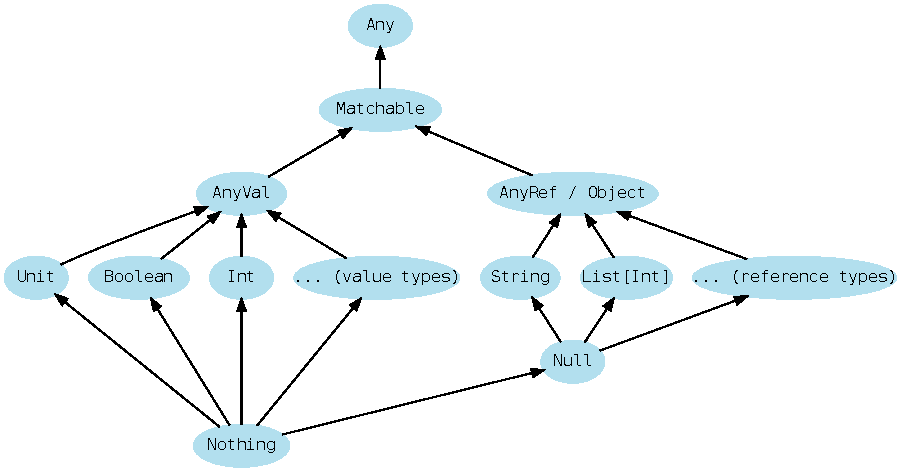
\includegraphics[width=\textwidth]{images/type-hierarchy}
    \caption{Scala 3 type hierarchy.}
    \label{fig:scala-type-hierarchy}
\end{figure}

Variance defines the rules on how the subtype relationships between parameterized types are dependent on the subtype relationship on the type on which it is parameterized. Variance has three variants: \emph{invariance}, \emph{covariance}, and \emph{contravariance}. Invariance means that subtyping relationships present in type parameters are not applied to the parameterized type at all. Covariance states that the subtype relationship of the parameterized type are in the same direction as a type parameter's subtype relationship. Contravariance means that the subtype relationship between parameterized types are the opposite way compared to the subtype relationships of the type parameter. When \inlinecode{Sub} is a subtype of \inlinecode{Super} and \inlinescala{F[_]} is any parameterized type, then
\begin{itemize}
    \item Under covariance, \inlinescala{F[Sub]} is a subtype of \inlinescala{F[Super]};
    \item Under contravariance, \inlinescala{F[Super]} is a subtype of \inlinescala{F[Sub]}; and
    \item Under invariance, \inlinescala{F[Sub]} and \inlinescala{F[Super]} have no subtyping relationship.
\end{itemize}

Covariance is applicable in parameterized types that contain, store, or produce values, in other words the type parameter is in covariant position. Contravariance is applicable in the opposite situation, where values of the type parameter are consumed, i.e. the type parameter appears in a function parameter list, and is said to be in contravariant position. Invariance is useful in situations where it does not make sense for the parameterized type to have inheritance based on type parameter, or when the parameterized type is a mutable, or the type parameter appears both in covariant and contravariant positions. A parametric type with multiple type parameters could declare each type parameter with different variance, for example functions in Scala are contravariant in their input type(s) and covariant in their result type.

An infamous example of a mutable covariant type is the primitive array type in Java and C\#.
These arrays must perform a runtime type check when adding elements to the array, and throw an exception if the type of the element is not compatible with the array, as demonstrated in \refsource{mutable-covariance}. To avoid these mandatory costs and checks, mutable collections in Scala are invariant. Immutable collections and containers, such as \inlinecode{Option} or \inlinecode{Either} are covariant in Scala.

\begin{algorithm}

\begin{minted}{java}
String[] a = new String[1];	
Object[] b = a; // String is a subtype of Object, so this is legal
b[0] = 1; // Runtime exception since cannot add Integer to String[]
\end{minted}

\caption{Covariance in mutable types, like Java primitive array, is problematic \label{mutable-covariance}}
\end{algorithm}

Programming languages differ in the way variance annotations are defined and used. Variance annotations in C\# and Scala are with the parameterized type. On the other hand, in Java one defines variance only when using a parameterized type. The former is called \emph{declaration-site} variance, demonstrated in \refsource{declaration-site-variance} and the latter is called \emph{use-site} variance, demonstrated in \refsource{use-site-variance}. Approaches deviating from these exist, for example TypeScript tries to infer variance, but it has optional declaration-site annotations from version 4.7 onwards. Kotlin has declaration-site variance by default but it emulates some parts of use-site variance with type projections.

\begin{algorithm}

\begin{minted}{scala}
class Invariant[A]      // Invariance is the default
class Covariant[+A]     // Covariance denoted with +
class Contravariant[-A] // Contravariance denoted with -
\end{minted}

\caption{Scala uses declaration-site variance, where the variance of a parameterized type is denoted in its type definition  \label{declaration-site-variance}}
\end{algorithm}

\begin{algorithm}

\begin{minted}{java}
interface Supertype {}
interface Subtype extends Supertype {}

void invariant(List<Supertype> list) {
    /* Get and set list values */
}
void covariant(List<? extends Supertype> list) {
    /* Only get list values */
}
void contravariant(List<? super Subtype> list) {
    /* Only set list values */
}
\end{minted}

\caption{Java has use-site variance, where the desired variance is declared when using the parameterized type \label{use-site-variance}}
\end{algorithm}

Invariance is the default in Scala and it does not require an explicit annotation. Covariance is declared with a \inlinecode{+} sign before each type parameter. Since contravariance could be seen as the opposite of covariance, it is denoted with a \inlinecode{-} sign.

Many features and principles from functional programming are not only available, but also encouraged in Scala. Pattern matching, first-class functions (\refsource{scala:lambdas}), and tail recursion are all supported and heavily utilized in idiomatic Scala programs. Immutable variables, collections and data-structures are the default way of writing Scala, even though mutable counterparts are also available. Functional data modeling is achieved with the use algebraic data types built into the language. Even though Scala embraces functional programming and imperative code is generally discouraged, introducing arbitrary side effects is possible.

\begin{algorithm}
\begin{minted}{scala}
val ns = List(1, 2, 3)

val mapped1 = ns.map(n => n + 1)
val mapped2 = ns.map(_ + 1) // Same as above in shorter form

val sum1 = ns.foldLeft(0)((x, y) => x + y)
val sum2 = ns.foldLeft(0)(_ + _) // Same as above in shorter form
\end{minted}

\caption{Long and short form of anonymous functions in Scala. \label{scala:lambdas}}
\end{algorithm}

In addition to ordinary functions, Scala has a specific function type called \\\inlinecode{PartialFunction} for representing functions that are not defined for all values of their input types. It is a subtype of the (normal) function type, to which it adds the method \inlinecode{isDefinedAt}, which must be used to check before every function call whether the function is defined for the given value. \refsource{scala:partial-function} shows how to define and use partial functions.

\begin{algorithm}
\begin{minted}{scala}
val someEvensMultipliedByTen: PartialFunction[Option[Int], Int] = {
  case Some(n) if n % 2 == 0 => n * 10
}

val opts  = List(None, Some(2), None, Some(3), Some(4))
val somes = opts.collect(someEvensMultiplied) // List(20, 40)
\end{minted}

\caption{Partial functions in Scala. \label{scala:partial-function}}
\end{algorithm}

Some functional languages, such as Haskell, have a special syntax for monadic computations. Scala also provides this syntactic sugar in a form of \inlinecode{for} comprehensions, demonstrated in \refsource{monad:for-syntax}. For comprehension is compatible with any data type that has \inlinecode{map} and \inlinecode{flatMap} methods defnied, such as \inlinecode{Option}, \inlinecode{Either}, and \inlinecode{ZIO} (Chapter \ref{zio}). These required methods can be added to any type by using extension methods.

Extension methods, which allow adding methods to a class separately from its definition, are one of Scala's more advanced features. Other state-of-the-art features of Scala include operator overloading and infix operator- and method syntax, higher kinded and dependent types, type lambdas, as well as powerful meta programming capabilities. Scala 3 introduced more cutting edge features such as automatic type class derivation and union and intersections types.

Probably the most distinguishing feature in Scala is its system of implicits and other contextual abstractions arising from that. A function can mark some of its parameters as implicit and the compiler will try to figure out that parameter from the enclosing scope by its type without programmer explicitly passing an argument for that parameter. Originally implicit parameters were introduced to achieve similar behavior as Haskell's type classes. Implicits can, however, also be used for other purposes, such as implicit conversions, context propagation, extension methods, and proving subtyping relationships between generic type parameters at compile-time.~\cite{tc-as-objects}

Syntactically to use implicits, a function can mark some of its parameters as implicit with the keyword \inlinecode{using}. When the function is called, the compiler tries to find a value marked as implicit, with the keyword \inlinecode{given}, from the enclosing scope. If all requested values are found, they are automatically applied as arguments. If any of the implicit parameters is not found, compilation error is reported. \refsource{scala:implicits} shows the function \inlinecode{summon} that searches for an implicit value by type, demonstrating the definition and use of implicit parameters.

\begin{algorithm}
\begin{minted}{scala}
case class Person(age: Int, name: String)

// Define type class
trait Show[A]:
  extension (a: A) def show: String

// Define type class instance
given Show[Person] with
  extension (a: Person)
    def show: String = s"${a.name} is ${a.age} years old"

// Use the type class
def showAll[A: Show](as: List[A]): List[String] =
  as.map(a => a.show)
\end{minted}

\caption{Implicits could be used to encode type classes \label{scala:typeclasses}}
\end{algorithm}

Another advanced feature utilizing implicit resolution is the ability of the Scala compiler to prove type equality or subtype relationships. The class \inlinescala{=:=[From, To]} is for type equality and \inlinescala{<:<[From, To]} for subtype relationship. Both classes extend a function \inlinescala{From => To}, and can be used to transform types. Types with two type parameters could be used as infix in Scala, for example type equality could be written \inlinescala{A =:= B}. When requesting an implicit parameter of either of the types above, Scala compiler synthesizes an instance if the type relationship holds, otherwise reports a compilation error. The act of proving type relationships is said to be \emph{witnessing}, and a common practice is to name the implicit parameter as \emph{evidence}. The feature is useful, for example, when defining functions that make sense only for specific types, as demonstrated in \refsource{scala:witness}, where only nested \inlinecode{Maybe} types could be flattened.

\begin{algorithm}
\begin{minted}{scala}
enum Maybe[+A]:
  case Just(a: A)
  case Nothing

  def flatten[B](using evidence: A <:< Maybe[B]): Maybe[B] =
    this match
      case Just(a) => evidence(a)
      case Nothing => Nothing

Maybe.Just(Maybe.Just(1)).flatten // Compiles
Maybe.Just(1).flatten // Error: Cannot prove that Int <:< Maybe[B]
\end{minted}

\caption{Scala compiler can prove (witness) a subtype relationship by providing implicit evidence. \label{scala:witness}}
\end{algorithm}

Another thing that sets Scala 2 and 3 apart is the introduction of intersection and union types in Scala 3. Intersection types are denoted with the \inlinecode{&} symbol and union types with \inlinecode{|}. Intersection \inlinescala{A & B} means that the resulting type has properties of both \inlinecode{A} \textbf{and} \inlinecode{B}. Union is the dual of intersection, and the resulting type of \inlinescala{A | B} is either \inlinecode{A} \textbf{or} \inlinecode{B}.

Intersection types are commutative, idempotent, and have \inlinecode{Any} as the identity element. Commutativity means that the order of types included in the intersection does not matter --- Scala considers permutations equal. Idempotency means that type intersectioned with itself is equal to the type itself. \inlinecode{Any} as the identity element means that the intersection of any type \inlinecode{A} with \inlinecode{Any} is equal to \inlinecode{A}, since all types themselves are subtypes of \inlinecode{Any}. Expressed as code, laws of intersection types can be proved with the Scala compiler:
\begin{itemize}
    \item Commutativity: \inlinescala{summon[(A & B) =:= (B & A)]}
    \item Idempotency: \inlinescala{summon[A =:= (A & A)]}
    \item Identity: \inlinescala{summon[A =:= (A & Any)]}
\end{itemize}

Like intersection types, also union types are commutative, idempotent, and obey the identity laws. The identity element is \inlinecode{Nothing}: the union of any type \inlinecode{A} with \inlinecode{Nothing} is equal to \inlinecode{A}, since there are no values of type \inlinecode{Nothing}. Again expressed as code, the laws of union types proved by the Scala compiler are:
\begin{itemize}
    \item Commutativity: \inlinescala{summon[(A | B) =:= (B | A)]}
    \item Idempotency: \inlinescala{summon[A =:= (A | A)]}
    \item Identity: \inlinescala{summon[A =:= (A | Nothing)]}
\end{itemize}
